\chapter{Background}
\label{chap:background}
In this chapter, we provide some usage examples for
glossaries and acronym lists with \texttt{glossaries} (Section \ref{sec:gloss}),
bibliography and citations with \texttt{biblatex} (Section \ref{sec:bib}), and more.

\begin{figure}[H]
    \centering
    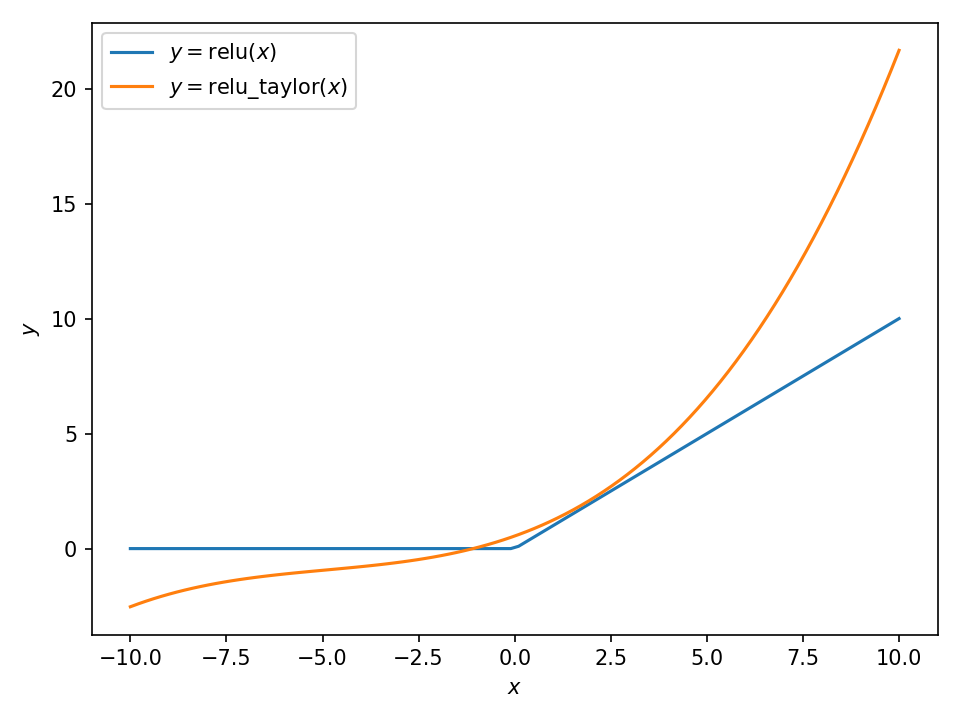
\includegraphics[width=0.8\linewidth]{figures/taylor-relu.png}
    \caption{Comparison of the Relu activation function vs. its Taylor expansion}
\end{figure}

\section{Notation and Acronyms}
\label{sec:gloss}
Symbols and acronyms are defined in the preamble, after loading the \texttt{glossaries} package, and used as follows.

In this chapter, we introduce the necessary background on the \gls{aes}.
We denote binary exclusive-or by \gls{xor}.

\section{Citations}
\label{sec:bib}
This is an example of how to specify and cite
a book \cite{AESbook},
a journal article \cite{bstjShannon49},
a conference article \cite{spKocherHFGGHHLM019},
and an informal report \cite{iacrSchneierFKR15}.
We can also add the authors' names to the citation:
\Gls{aes} is a block cipher defined by \textcite{AESbook}.
